\chapter{Experimental Setup}
\label{ch:exp}

All data analysed in this thesis was recorded with the CMS experiment at the Large Hadron
Collider (LHC) at the European Organization for Nuclear Research (CERN) near Geneva, Switzerland.
This chapter provides a short overview of CERN and its accelerators, the LHC, as well as a
short description of the main components of the CMS experiment.

\section{The Large Hadron Collider}
\label{sec:lhc}
The LHC \cite{lhc_designreport} is currently by far the largest and most powerful particle accelerator in
the world. It is a circular accelerator situated in a tunnel around 100 metres below the Swiss-French
border west of Geneva. Its main purpose is accelerating protons to energies of up to 13 TeV
\footnote{One electronvolt (eV) is the energy acquired by a charge of 1$e$ passing through an electric field of 1 volt, equivalent to \num{1.602e-19} Joule.} 
in the final development stage of the machine starting in 2015. 
Besides the acceleration of protons it is also capable of accelerating heavy ions (predominantly lead ions) to energies of up to 
2.76 TeV per nucleon.

\subsection{The acceleration chain}
\label{sub:chain}
Particles injected into the LHC for final acceleration are required to have an energy of 450 GeV. This is
achieved by a long chain of linear and circular accelerators, a sketch of which can be seen in
Fig.~\ref{fig:accelerators}. 

\begin{figure}[h!]
    \centering
    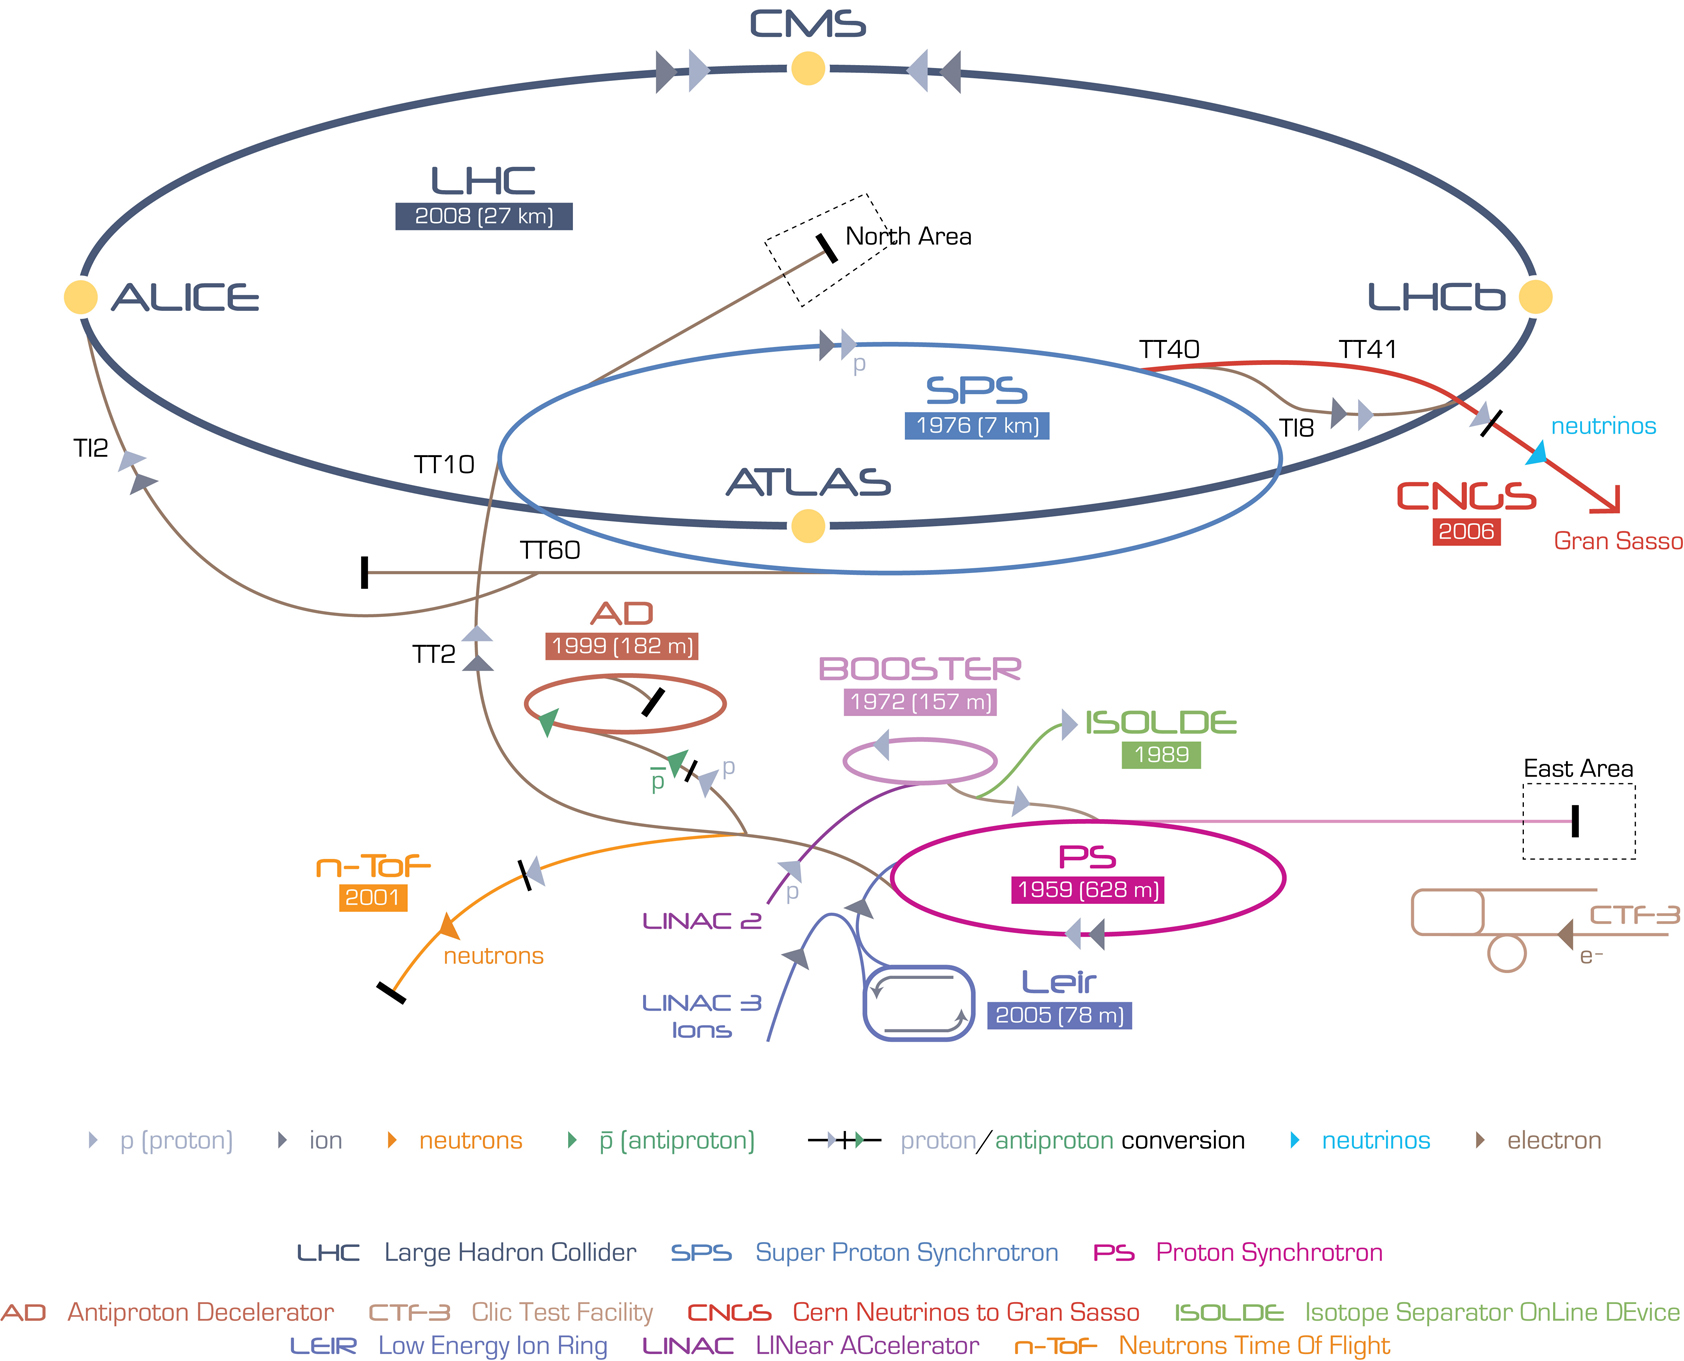
\includegraphics[width=0.65\textwidth]{../figs/Cern-Accelerator-Complex.jpg}
    \caption{Conceptual drawing of all accelerators and experiments hosted at CERN. Besides operating
    the LHC, there are many other accelerators, decelerators and experiments being operated.}
    \label{fig:accelerators}
\end{figure}

Protons used for acceleration in the LHC are extracted from a hydrogen molecules in a bottle situated 
at the CERN main site. These molecules are stripped of their electrons by strong electric fields
and subsequently injected into the first acceleration stage, the linear accelerator Linac 2. Upon exiting
Linac 2, the protons have gained an energy of 50 MeV and are injected into the first circular accelerator,
the Booster. This synchrotron with a circumference of 157 meters accelerates the protons to an energy of 1.4 GeV and
uses magnetic dipole fields to bend the protons onto a circular path. These bending magnets are operated at 
room temperature for the Booster and in fact all the accelerators up to the LHC.
From the Booster, the protons are injected further into the Proton Synchrotron, an accelerator originally built
in 1959 with a circumference of 628 meters and an output energy of 25 GeV. The last step before injection into
the LHC is the Super Proton Synchrotron (SPS), which accelerates the protons to the LHC injection energy of 450 GeV.
The SPS is the world's second largest accelerator with a circumference of nearly 7 km, and it was the first accelerator
to collide protons and anti-protons at energies high enough to produce $W$ and $Z$ bosons, leading to their discovery in 1983
\cite{Wdiscovery, Zdiscovery}.

Ions pass through the same accelerators on their way to the LHC with the notable exception of the very first 
acceleration being done in Linac 3 rather than Linac 2.

While the LHC is filled and delivering collisions to its experiments, the accelerators are used to provide
particles to other experiments ongoing at CERN. The Antiproton Decelerator (AD) in which anti-protons are 
decelerated and combined with positrons to form anti-hydrogen, and the ISOLDE collaboration for the study
of many different radioactive ions are just some of the examples of interesting experiments ongoing at CERN.

\subsection{Specifications of the LHC}
\label{sub:lhc}
The LHC itself is located in a tunnel roughly 50-150 meters below ground in the Geneva
area, extending from Lake Geneva all the way to the Jura mountain chain. Its total circumference is \num{26659} meters
which makes it -- together with its predecessor the Large Electron Positron Collider hosted in the same tunnel -- by 
far the largest particle accelerator ever built. It is divided into 8 sectors, separated and named by the eight access
points to the tunnel. A schematic drawing of the LHC with all its access points can be found in Fig.~\ref{fig:lhc_scheme}.
Access points 1, 2, 5, and 8 host the four main experiments ATLAS, ALICE, CMS, and LHCb, the acceleration is performed
by radio-frequency (RF) cavities at point 4, the beam-dump system is located at point 6 and beam monitoring
and conditioning is performed at points 3 and 7~\cite{cmsdetector}.

\begin{figure}[h!]
    \centering
    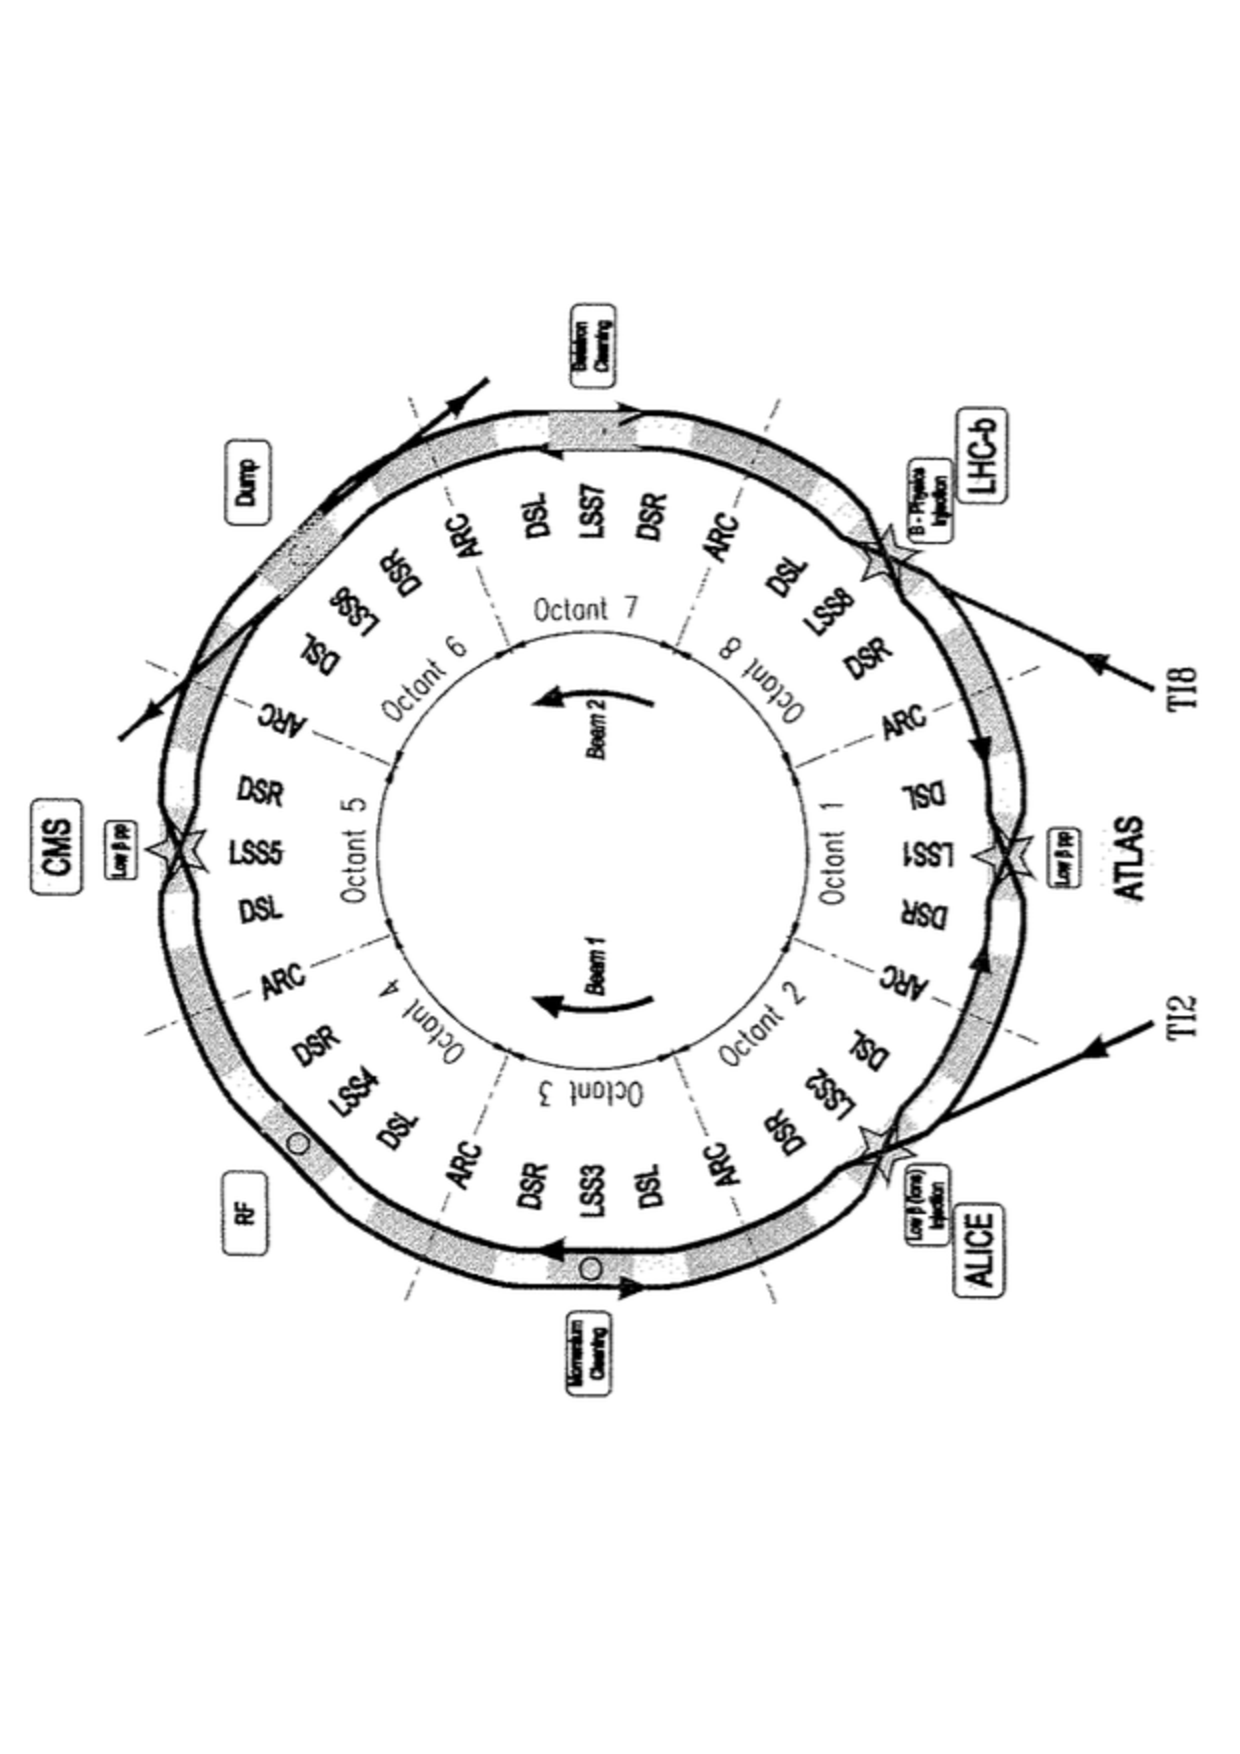
\includegraphics[width=0.65\textwidth]{../figs/lhc_scheme.pdf}
    \caption{Schematic drawing of the LHC ring and its sectors and access points numbered in clockwise direction
    starting at the ATLAS experiment in point 1.}
    \label{fig:lhc_scheme}
\end{figure}


\subsubsection*{The magnet system}
Particles are injected from the SPS into the LHC into two counter-rotating beams in discrete bunches
at the aforementioned 450 GeV. In order to control the particles on their circular path, an intricate magnet 
system was designed in order to bend and to focus the beams. The main feature of the LHC magnet system are
the 1232 dipole bending magnets, each roughly 15 meters in length and weighing 30 tonnes. These magnets
are made of a niobium-titanium alloy, a type-2 superconductor which allows current transport without loss
at the operating temperature of 1.9 K. Cooling of the LHC cold mass of roughly 37 Mt is achieved with pressurized superfluid helium. 
Each magnet hosts two separate beam-pipes for beam 1 (clockwise) and beam
2 (counter-clockwise) with the dipole magnetic field pointing in opposite direction in either of them. In order to achieve
acceptable beam lifetimes and to minimize beam-gas interactions, the beam pipes are evacuated and the residual gas
pressure is around \num{e-10} mbar.
Upon injection from the SPS the dipole magnets are operated at a magnetic field strength of 0.535 T which is slowly
raised during the acceleration period of the beam to a final field strength of 8.33 T at the maximum collision
energy.

Alongside the dipole magnets for the bending of the particles, there are thousands of additional magnets for correcting
and controlling the particle's path. The largest part of the correction magnets are sextupole magnets situated
on either side of every dipole magnet. Further components include a decapole and an octupole corrector for
each dipole magnet as well as injection kicker magnets and kicker magnets for the beam dump system among others.

\subsubsection*{The RF cavities}
Once the LHC is filled and circulation of the beams is stable, they are accelerated from their initial energy
by the means of so-called RF cavities which provide a high frequency alternating electric field of nominally
400.8 MHz. Similar to the bending magnets, the RF cavities are operated in a superconducting state at a temperature
of 1.9 K.
There are a total of eight such cavities per beam, each achieving a potential difference of 2 MV for a combined 16 MV 
necessary for acceleration at collision energy. During the acceleration period of the beams, the energy gain
per particle per turn is 485 keV with the total power consumption of the RF system being around 275 kW. 

\subsubsection*{Beam parameters}
In order to measure the performance of a particle accelerator such as the LHC, the quantities of instantaneous and integrated
luminosity are the most important figure of merit, as they correspond to the total number of particle collisions
produced in any given collision point. The instantaneous luminosity is defined as

\begin{equation}
    L = \frac{N_b^2 n_b f_{rev} \gamma_r}{4 \pi \epsilon_n \beta^*} F,
\end{equation}
where $N_b$ denotes the number of particles per bunch, $n_b$ the number of bunches per beam, $f_{rev}$ the revolution 
frequency of each bunch, $\gamma_r$ the relativistic gamma factor, $\epsilon_n$ the normalized beam emittance,
$\beta^*$ the $\beta$-function of the beam at the collision point, and $F$ a geometrical factor inversely proportional
to the crossing angle of the two beams at the interaction point. 

The beam emittance is defined as the 
volume of the beam in the position-momentum phase space and is thus a measure of the quality of the beam. Emittance itself is 
inversely proportional to the beam momentum and it is therefore necessary to introduce a normalized emittance, which does not change
its value with momentum in order to compare beam quality before and after acceleration. The $\beta$-function describes the
behavior of the transverse beam size as a function of the position in the accelerator, and the value $\beta^*$ is consequently
proportional to the transverse size of the beam at the collision point.

The dimension of the instantaneous luminosity is $cm^{-2}s^{-1}$ and by integrating it over time
the integrated luminosity $\mathcal{L}_{int}$ is obtained. Through knowledge of the latter, one can calculate the total number
of expected events for any given physical process in a data sample of a given size by
\begin{equation}
    N_{\text{process}} = \mathcal{L}_{int} \cdot \sigma_{\text{process}}.
\end{equation}

All relevant beam parameters to calculate the instantaneous luminosity at the LHC are summarized in Table~\ref{tab:lhc}
at both injection and collision energies. 

\begin{table}
    \begin{center}
    \caption{Beam parameters for beams in the LHC at injection and collision energy.}
    \label{tab:lhc}
    \begin{tabular}{ r l | c | c }
    \multicolumn{4}{c}{\textbf{Beam parameters}} \\                                                                                            \hline
                                                                & Unit         & Injection                                    & Collision \\   \hline \hline
    Beam Energy                                                 & [GeV]        & 450                                          & 3500 - 7000 \\ \hline
    Relativistic $\gamma_r$                                     &              & 479.6                                        & 3730-7461  \\  \hline
    Particles per bunch                                         &              & \multicolumn{2}{c}{\num{1.15e11}} \\                          \hline
    No. of bunches                                              &              & \multicolumn{2}{c}{2808} \\                                   \hline
    $f_{rev}$                                                   & [Hz]         & \multicolumn{2}{c}{11245}                            \\       \hline
    $\epsilon_n$                                                & [$\mu$m rad] & 3.5                                          & 3.75 \\        \hline
    Half crossing angle\footnote{\label{note1}at CMS and ATLAS} & [$\mu$rad]   & $\pm$ 160                                    & $\pm$ 142.5 \\ \hline
    $\beta^*$                                                   & [m]          & 18                                           & 0.55 \\        \hline %\footnotemark[\ref{note1}]
%    Beam energy per beam [MJ] & 23.3 & 362 \\ \hline
%    Synchrotron radiation per ring [W]& \num{6.15e-2} & \num{3.6e3} \\ \hline
    \hline
    \end{tabular}
    \end{center}
\end{table}

\subsubsection*{Performance of the LHC}
All values in Table~\ref{tab:lhc} refer to the design values of the LHC, while the actual performance since startup in
2008 has been considerably different. After the initial startup in the autumn of 2008 when beams were first injected 
into the machine, a faulty connector between superconductors caused a significant explosion in the cooling system of the main magnets, resulting
in a shutdown and repair period until late 2009. However, upon restarting of the machine in 2009, operations of
the LHC have been almost flawless, with many parameters of the LHC reaching or even exceeding their design targets.
Since the limiting factor for the LHC energy is the attainable magnetic field strength in the bending magnet, combined with 
safety concerns regarding the replaced connectors from the incident in 2008, a staged approach for a slow energy ramp-up
was implemented for the LHC. First stable collisions for data-taking in 2010 were performed at an energy per proton
of 3.5 TeV resulting in 7 TeV center-of-mass energy. This energy was maintained also during 2011 before being increased
to 8 TeV in center-of-mass energy during the 2012 data-taking period. This thesis focuses on the dataset at 8 TeV.
The energy will further be increased to 13 TeV in center-of-mass in early 2015.

Regarding the luminosity, the LHC has outperformed its early expectations. Despite the fact that so far only
half the bunches were filled, resulting in a bunch spacing of 50 ns instead of the design 25 ns, the maximum
instantaneous luminosity has almost reached its design value of \num{1e34} $cm^{-2}s^{-1}$ in late 2012, when 
an LHC fill with an instantaneous luminosity of \num{7.67e33} $cm^{-2}s^{-1}$ was recorded. This was mostly
due to the increase in protons per bunch.

\subsubsection*{Pileup}
In order to reach the luminosities discussed in the previous section, it is necessary for the LHC to produce more than
one proton-proton collision per bunch crossing in the experiments. This effect is called pileup and poses great difficulty
to the experiments in handling the many interaction vertices. Since the total inelastic cross-section in the LHC is dominated by
rather unexciting, low-mass and low-energy very forward QCD interactions, it is very unlikely to observe more than one `interesting' 
proton-proton collision per bunch crossing. Nevertheless, some problems for the experiments associated with pileup include the identification of the `interesting' 
vertex, the assignment of electrically neutral particles to said vertex, energy corrections for detector objects such as jets, leptons,
and the missing momentum due to pileup interactions, and occupancy in the subdetectors. 

The number of proton-proton interactions per bunch crossing follow a Poisson-distribution of which the mean reached about 20 in 2012~\cite{pileupCMS}.


\section{The CMS experiment}
\label{sec:cms}
As briefly mentioned before, the LHC provides high energy particle collisions to four large particle physics experiments, namely
the ALICE, ATLAS, CMS, and LHCb experiments. While the ALICE and LHCb experiments are specially designed for specific purposes,
the study of heavy ion collisions and the study of processes involving the b-quark, respectively, the ATLAS and CMS experiments
are design as `general purpose' experiments. As such, their goal is the detailed scrutiny of the SM, the search for the recently observed
Higgs boson [FIXME - reference], and the search for new physics phenomena. They do this by means of measuring and absorbing decay products
of the collisions. The relevant physical observables of any particle produced in a particle collisions are the momentum vector
and the energy of a particle. Once these two quantities are known, every particle can be identified unambiguously. 

Data collected for this thesis were recorded by the CMS experiment.

\subsection{General structure and the magnet}
\label{sub:cms_general}
The Compact Muon Solenoid (CMS) experiment is located roughly 100 meters below ground in Cessy, France,
it is cylindrically shaped with dimensions of roughly 22 meters in length and a diameter of about 16 meters. 
The whole apparatus comprises a barrel part in the center and a so-called endcap on either side to seal the detector as hermetically as possible.
A drawing of the CMS detector is shown in Fig.~\ref{fig:cms_scheme}. 

\begin{figure}[h!]
    \centering
    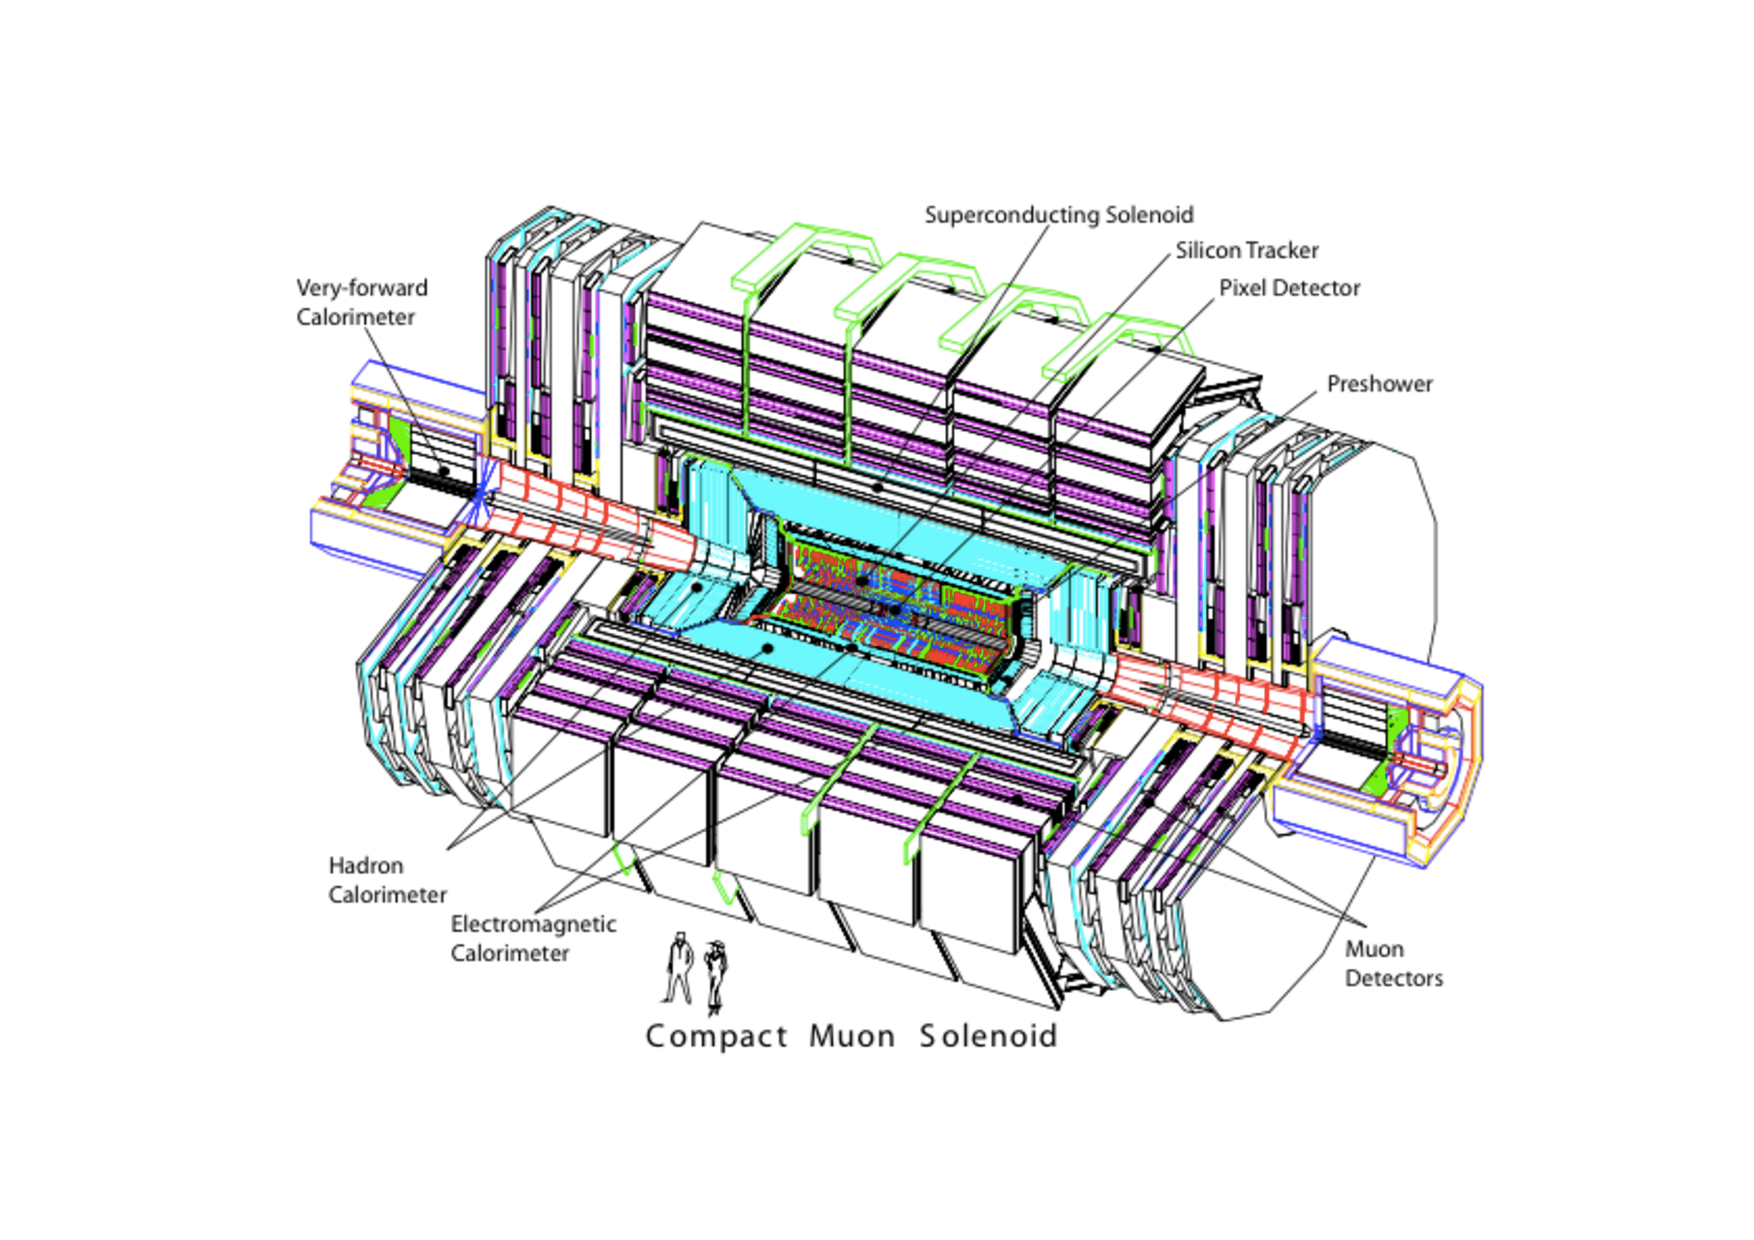
\includegraphics[width=0.85\textwidth]{../figs/cms_scheme.pdf}
    \caption{Perspective view of the CMS detector. The cylindrical shape as well as the barrel and endcap
geometry can be clearly seen. The depicted people are to scale~\cite{cmsdetector}.}
    \label{fig:cms_scheme}
\end{figure}

The convention for the coordinate system is as follows. The origin of the coordinate system is at the nominal
interaction point. The x-axis points towards the center of the LHC ring, the y-axis points towards the surface
and the z-axis points towards the west, along beam 2. The azimuthal angle $\phi$ is measured in the x-y plane, while the
polar angle $\theta$ is measured from the positive z-direction. It is commonly replaced by a quantity called 
pseudo-rapidity defined as $\eta = - \log \left[ \tan \left(\frac{\theta}{2} \right) \right]$.



As the presence of the word `solenoid' in the acronym for CMS already suggests, its main feature is a very large, solenoid
magnet which defines the overall structure of the experiment. Much like the LHC bending magnets, it is a superconducting
structure and the conducting material is a niobium-titanium alloy, albeit at a very different scale. It measures roughly six
meters in inner diameter and 13 meters in length, carrying a current of about \num{18000} (FIXME) ampere, resulting in a
maximum magnetic field strength of 3.8 T~\cite{magnettdr}. In addition to the actual magnet, the CMS magnet system
also comprises a return yoke for the magnetic field lines to be homogeneous as a function of the distance from the interaction
point. Altogether, the magnet system weighs approximately \num{11000} metric tons, by far the heaviest component of the 
CMS detector. As momentum resolution of charged particles is a critical factor in the physics performance of a detector, the magnetic
field strength within the tracking volume is desired to be as large as possible. 

The large volume of the CMS magnet allows for most sub-detectors to be situated within a very high magnetic field. Not only the
tracking detectors, but also the calorimetry for energy measurement are fully incorporated within the magnet's volume.



\subsection{The sub-detectors}
\label{sub:cms_subdet}
The structure of CMS is a layered, onion-like assembly of different sub-detectors. In the very center, the beryllium beam-pipe
passes through the detector with a diameter of 2.5 cm FIXME!!. Moving radially outwards from the center of the beam-pipe,
the layers are first the silicon pixel detector followed by the silicon strip tracker, the electromagnetic calorimeter,
the hadronic calorimeter, the superconducting magnet and finally the magnet return yoke interleaved with the muon chambers.

\subsubsection*{The CMS pixel detector}
The CMS pixel detector is a layered silicon detector with a pixel size of 100 $\times$ 150 $\mu m^2$ with the purpose of measuring the
trajectory of charged particles very precisely. It is divided into
a barrel (BPIX) and two endcap `forward' parts (FPIX) symmetrically arranged around the nominal interaction point. The BPIX comprises three
concentric layers of 53 cm in length and at radii of \num{4.3}, \num{7.2}, and \num{11} cm from the interaction point, while there are two FPIX 
disks on either side of the BPIX, at distances of z=$\pm$\num{34.5} and z=$\pm$\num{46.5} cm, extending from a radius of \num{6} to 15 cm.
In combination, the barrel and endcap part provide high granularity tracking up to a pseudo-rapidity of $\eta$ = 2.5, corresponding to a 
polar angle of roughly \ang{10}.
A sketch of both the pixel detector and the silicon strip can be found in Fig.~\ref{fig:tracker}.

\begin{figure}[h!]
    \centering
    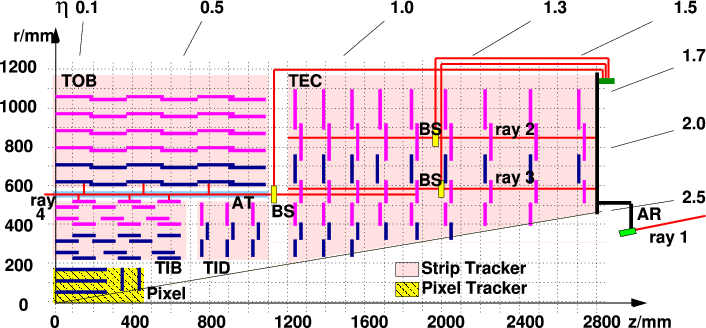
\includegraphics[width=0.85\textwidth]{../figs/tracker.png}
    \caption{Sketch of a quarter of all parts in the CMS tracking system with distances in radius $r$ and $z$. The pixel detector is close to the
interaction point shown in yellow, the silicon strip tracker is underlaid in pink. Each pink and blue solid line represents an active
detector layer~\cite{cmstrackeralignment}.}
    \label{fig:tracker}
\end{figure}

Both the FPIX and the BPIX are organized into single detector modules. There are 768 modules in the barrel part and 672 modules in the four
forward disks, each consisting of 2 to 16 readout chips (ROCs)~\cite{bpix}. Every ROC has a size of roughly 8$\times$8 \si{\square\milli\meter} and is bump-bonded
to an active silicon layer of 285 \si{\micro\meter} in thickness, divided into 52$\times$80 single pixels. In total, there are  1440 modules containing
about \num{16000} ROCs with a gross pixel count of about 66 million and a total silicon area of about one square meter. 
Such a high granularity is needed in order to obtain good spacial resolution
at the interaction point, good reconstruction of the tracks and in order to keep the occupancy low in high luminosity running of the LHC. At design
luminosity of \num{1e34} \si{\per\square\meter\per\second}, the CMS pixel detector is hit by about \num{1000} particles per bunch crossing, leading
to an occupancy of less than one percent.
Even with relatively low occupancies, the total flux of particles in the inner layers of the pixel detector are sufficiently high to induce
significant radiation damage. For this reason, the pixel detector has to be replaced during run 2 of the LHC, an event scheduled for late 2017.

\subsubsection*{The silicon strip tracker}
Just outside the pixel detector, further away from the interaction point lies the silicon strip tracker. Its purpose is much the same as the
pixel detector, albeit with a much larger covered area and a much smaller number of active channels. It occupies the radial distances from
20 to 116 cm and a length in z-direction of \si{5.8 \meter}. It is also divided into a cylindrical barrel part and endcap parts perpendicular to the beam direction. The naming scheme of the 
different parts is the Tracker Inner Barrel (TIB) and the Tracker Outer Barrel (TOB) for the layers parallel to the beam direction and the
Tracker Inner Disks (TID) and the Tracker EndCaps (TEC) for the perpendicular part. In total, there are \num{15148} single detector modules
in the silicon strip tracker\cite{siliconstrip} with varying sizes of strip widths and inter-strip pitch lengths. The inter strip pitch varies
from \si{80 \micro\meter} at low radius to \si{200 \micro\meter} at higher radius, while the ratio between pitch and width is constant at \num{0.25}.
The combined surface of the 9.3 million single channels is around \si{198 \square\meter}, making it the largest silicon tracker ever built.
The thickness of the silicon also varies between \si{320 \micro\meter} in the inner part of the detector and \si{500 \micro\meter} on the outside part. With this specifications,
the total occupancy at design luminosity is approximately 1\%. Altogether, a particle traversing the strip tracker will
hit about ten active silicon layers\footnote{This depends on the exact trajectory and varies between eight and 14 layers.}.

Due to the high granularity,
the multi-layered design, and the very high and homogeneous magnetic field in the tracking volume, the performance of the CMS tracking system
is impressive. Single point resolutions are around \si{30 \micro\meter} and in combination, the impact parameter resolution of is around 
around 10 \si{\micro\meter} for high energy muons, while the momentum resolution varies from around 1\% for low-\pt muons in the central
region to about 8\% for high-\pt muons in the forward region.

\subsubsection*{The electromagnetic calorimeter}
CMS has adapted a design with two separate calorimeters for electromagnetically and hadronically interacting particles. Both of those
calorimeters are contained within the superconducting magnet, as shown in a sketch of the CMS calorimetry in Fig.~\ref{fig:cms_calo}. 

\begin{figure}[h!]
    \centering
    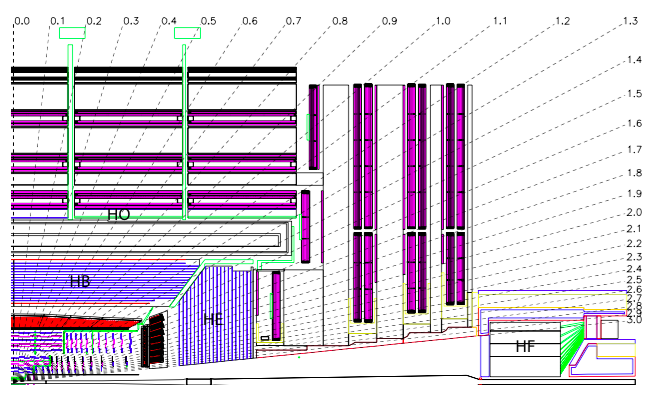
\includegraphics[width=0.85\textwidth]{../figs/cms_calo.png}
    \caption{Design of the CMS calorimetry system. The homogeneous electromagnetic calorimeter is shown in red towards
the center of the detector, while the hadronic calorimeter extends to larger radii~\cite{cmsdetector}.}
    \label{fig:cms_calo}
\end{figure}

The electromagnetic calorimeter (ECAL) is a homogeneous calorimeter made of \num{68524} lead tungstate (PbWO$_3$) crystals built to absorb and measure 
electromagnetically interacting particles such as photons and electrons. The material was chosen
for its mechanical and scintillating properties. With a density of 8.28 \si{\kilo\gram\per\cubic\meter} it has a very short radiation length of
0.89 \si{\centi\meter} as well as a small Moli\`{e}re radius of about 2.2 \si{\centi\meter}\footnote{The radiation length is the distance at which 
the energy of an incoming electron has decreased to $\frac{1}{e}\sim$37\% due to bremsstrahlung and about $\frac{7}{9}$ times the distance after which a high
energy photon would produce an $e^+e^-$ pair. The Moli\`{e}re radius defines the transverse containment of an electromagnetic shower.}
, allowing for a high granularity and adequate spacial resolution of electromagnetic showers. Its scintillating properties
include a very short signal collection time of about 25 \si{\nano\second} for 80\% of the signal and a relatively low photo-electron output of
4.5 per \mev in a wavelength spectrum with a broad maximum in the blue-green 420-430 \si{\nano\meter} region. This light is collected
and amplified by photo-multipliers which are mounted to the rear end of the crystals.
Each crystal has an area of 22$\times$22 \si{\square\milli\meter} on the front facing side and 26$\times$26 
\si{\square\milli\meter} on the far side, corresponding to a spacial resolution of 0.0174$\times$0.0174 in  $\eta$-$\phi$. The length 
in radial direction is 230 \si{\milli\meter}, corresponding to \num{25.8} radiation lengths. The barrel part of the ECAL (EB) extends to 
$|\eta|$ = 1.479, and the endcap part (EE) covers the pseudorapidity range from 1.479 $<$ $|\eta|$ $<$ 3.0.

The energy resolution of a calorimeter can be parametrized by
\begin{equation}
\label{eq:calo_res}
    \left( \frac{\sigma}{E} \right) =   \left( \frac{\text{a}}{\sqrt{E}} \right)   \bigoplus  \left( \frac{\text{b}}{E} \right)  \bigoplus  \text{c} ,
\end{equation}
where $a$ is called the stochastic term, $b$ the noise term, and $c$ a constant term. At low particle energies both the stochastic term and the 
noise term dominate the resolution, while at higher energies the importance of the constant term becomes more important.
From measurements in testbeams, the terms for the energy resolution of the CMS ECAL were found to be
\begin{align*}
    a &= 2.8 \%, \\
    b &= 12.0 \%, \\
    c &= 0.3 \% ,
\end{align*}
for the energy in \gev~\cite{ecalresolution}. For the most relevant physical processes, such as $H\rightarrow\gamma\gamma$ or $Z\rightarrow e^+e^-$, the total resolution
both for electrons and photons is of the order of 1\% in the central part and of the order of a few percent in the
forward part of the detector.

\subsubsection*{The hadronic calorimeter}
For an accurate measurement of the missing transverse energy or momentum, a precise knowledge of the energy of hadronic jets is of 
paramount importance. However, since the available volume within the CMS magnet is limited, a compromise on the hadronic calorimeter (HCAL)
had to be made. The implemented design is a sampling calorimeter, interleaved layers of a massive passive absorber material and a lighter,
but active scintillating material. The task of the passive absorber is to create particle showers, which can then be measured in the active
material. 

The geometry is again divided into a barrel (HB) and an endcap (HE) part. The HB consists of two steel plates as first and last absorber layer and
14 layers of brass of variable thickness in between. In total, these 16 layers of absorber material in the barrel amount to 5.82 interaction lengths
\footnote{An interaction length corresponds to the mean distance at which a hadronic particle undergoes a nuclear interaction.} 
of material at $\eta$ = 0 up to 10.6 interaction lengths at $|\eta|$ = 1.3. The HE
is composed of 18 brass absorber plates constituting about 10 interaction lengths along the coverage up to $|\eta|$ = 3.0.
Every absorber plate is combined with a layer of plastic scintillator organized in tiles each occupying an area of 0.087$\times$0.087, which drives 
the spacial resolution of the hadronic calorimeter. In addition to the components contained within the superconducting magnet, the hadronic calorimeter
features another layer of detector material just outside the magnet, called the hadronic outer (HO) in order to measure hadronic jets with an energy
sufficient to traverse the HB and the magnet (so-called punch-throughs). There is also a hadronic calorimeter for high-$\eta$ jets, called the hadronic forward (HF) covering 
pseudo-rapidities of 3.0 $<$ $|\eta|$ $<$ 5.0.

Since the HCAL is a sampling, rather than a homogeneous, calorimeter involving large parts of inactive material, its energy resolution is significantly
worse than the one of the ECAL. Adding to this lower precision is the fact that hadronic interactions are accompanied by some unmeasurable energy 
losses in nuclear excitations. Using the same parametrization as in Eq.~\ref{eq:calo_res}, the parameters for the HCAL are found to be
\begin{align*}
    a &= 1.25, \\
    b &= 5.6, \\
    c &= 0.033.  
\end{align*}
For relevant hadronic jets in analyses for SUSY and most other use-cases, the resolution takes values of about 25 \% for 40 GeV jets and decreases
with energy to values of about 10 \% or less at energies of jets above 100 GeV.

\subsubsection*{The muon system}
As the acronym CMS already suggests, special emphasis in the design of the detector was put into designing and constructing a system
which is capable of measuring muons with a very high precision in order to be sensitive to high-sensitivity processes such as
the Higgs boson decaying into four leptons. This is achieved by three types of gaseous detectors encased in the return yoke of the magnet, namely
the Drift Tubes (DTs) in the barrel part, Cathode Strip Chambers (CSCs) in the two endcap parts, and a set of fast Resistive Plate Chambers (RPCs) 
used for triggering on muons and timing. The total coverage can be expressed by the reconstruction efficiency as a function of the pseudo-rapidity,
which achieves values close to 100 \% all from values of 0. $<$ $|\eta|$ $<$ 245, with a notable exception at around $|\eta|$ = 0.25, and $|\eta|$ = 0.8, where it
drops to around 94 \% and 97 \%, respectively, due to small gaps between the DTs. The layout of the muon system can be seen in Fig.~\ref{fig:muons}, where 
a quadrant of the CMS detector is shown.

\begin{figure}[h!]
    \centering
    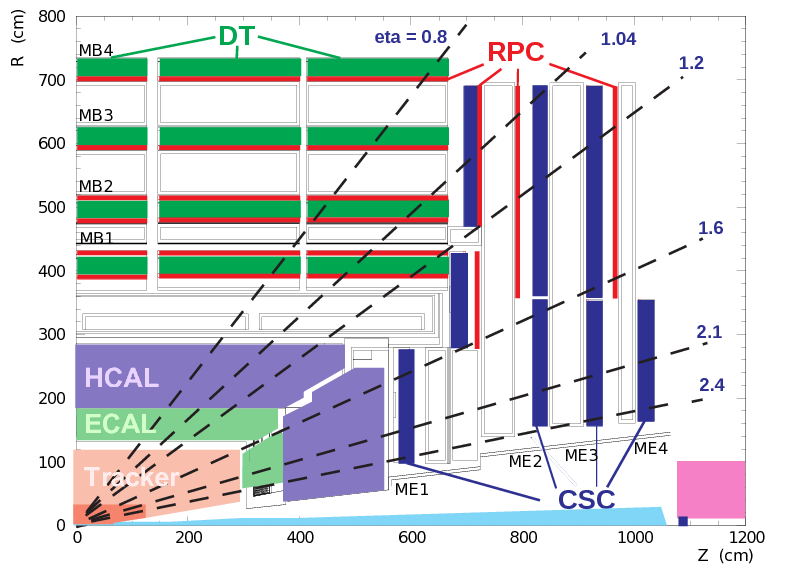
\includegraphics[width=0.85\textwidth]{../figs/muon_system.png}
    \caption{Layout of the CMS muon system. The DTs comprise the barrel part of the detector, while the CSCs are exclusively
situated in the endcap part. RPCs are attached to both types of detectors for triggering and timing measurements~\cite{muonsystem}.}
    \label{fig:muons}
\end{figure}

The DTs are organized in four concentrical cylinders in the barrel part with a total of 250 drift chambers containing \num{172000} active wires.
They are made of multiple so-called superlayers, which are essentially stacked tubes either in beam direction or perpendicular to it. Two or three
of those superlayers are then combined into one DT, with altering orientation of the wires to provide maximum spacial resolution. RPCs are glued to the DTs, on both sides for the
inner two cylinders and on the inner side for the outer two. The gas in the 
drift tubes is a mixture of 85\% Ar and 15\% CO$_2$ and the drift length is chosen to be 21 \si{\milli\meter} with a drift time of roughly 380 \si{\nano\second},
allowing for negligible occupancy.

Because of the much higher flux and an inhomogeneous magnetic field in the forward part of the detector, a different detector design had to be chosen for high values of $|\eta|$.
The CSCs are a set of 468 trapezoidal modules, each covering from \ang{10} to \ang{20} in $\phi$. Each CSC consists of six gas-filled gaps with cathode strips running radially
and anode wires running almost perpendicular to the strips. The $r$, $\phi$, and $z$ coordinates of a traversing muon is thus measured six times per CSC, and there
are in total four layers of CSCs in each endcap. There are a total of \num{220000} readout channels of the strips and another \num{180000} readout channels of the wires,
allowing for good spacial resolution and low occupancy even at high flux rates of up to 1 \si{\kilo\hertz\per\square\centi\meter} at full LHC luminosity. The gas mixture
is 40\% Ar, 50\% CO$_2$, and 10\% CF$_4$, where the CO$_2$ component achieves a high signal gain, while the CF$_4$ component protects the wires from polymerisation. Three
layers of RPCs are connected to the CSCs in the outer part of the endcap.

RPCs are gas-filled detectors which have a very fast signal rise-time, comparable to that of scintillators. Since the time resolution is much better
than the LHC bunch spacing of 25 \si{\nano\second}, the RPCs provide not only an accurate estimate of the momentum of a muon, but also unambiguous
assignment to a bunch crossing. Each RPC is made up of two 2 \si{\milli\meter} wide, gas-filled gaps with strips on the common side and plates of plastic on the outer sides. These 
simple circuits are operated in avalanche mode in order to ensure good operation at high rates.

Using the three muon-subsystems and combining their measurement, a standalone muon momentum resolution of below 10\% can be achieved for muons up to 200 GeV. This value increases
to between 15\% and 40\% for muons of 1 TeV momentum, depending on the position in $|\eta|$. Since a muon can be identified also in the tracker volume, 
combining the tracks from the inner part of the detector with the information of the muon chambers improves this resolution to roughly a percent for momenta below 200~GeV and
about 5\% for momenta of 1 TeV.

\subsection{The trigger system}
\label{sub:cms_trigger}
With a bunch crossing frequency of \SI{40}{\mega\hertz} and a mean number of collisions per bunch crossing of roughly 20, there are up to 800 million collisions taking
place inside CMS every second. Considering that the whole of CMS has roughly 100 million readout channels, this would lead to unsustainable data-rates, even for the most 
powerful readout and network possible to date. For this reason, a triggering system has been implemented in order to differentiate `interesting' collisions from those
who are considered not. CMS has adopted a two-stage approach, with a first, hardware-based and thus very fast triggering mechanism called the Level-1 trigger (L1), followed
by a second, fully software based trigger named the High-Level-Trigger (HLT). 

\subsubsection*{The L1 trigger}
Dealing with complicated data at a rate of \SI{40}{\mega\hertz} requires for processing of information at speeds that are unattainable for software reconstruction. 
Therefore, a fully hardware based system has been implemented, relying heavily on the use of integrated circuits in the form of so-called Field-Programmable-Gate-Arrays (FPGAs).
Because speed is such an important point of the triggering decision, not all information from the detector can be used in order to make a yes/no decision on an event-by-event
basis. In the current L1 trigger system, only coarsely segmented information from the calorimeters and the muon system are used for the trigger decision, 
while the full data from the muon system, the calorimeter, and the silicon tracker are stored in buffers until a trigger accept (L1 accept) triggers the full readout of these buffers.
An organizational sketch of the different participants for a trigger decision is shown in Fig.~\ref{fig:l1}
\begin{figure}[h!]
    \centering
    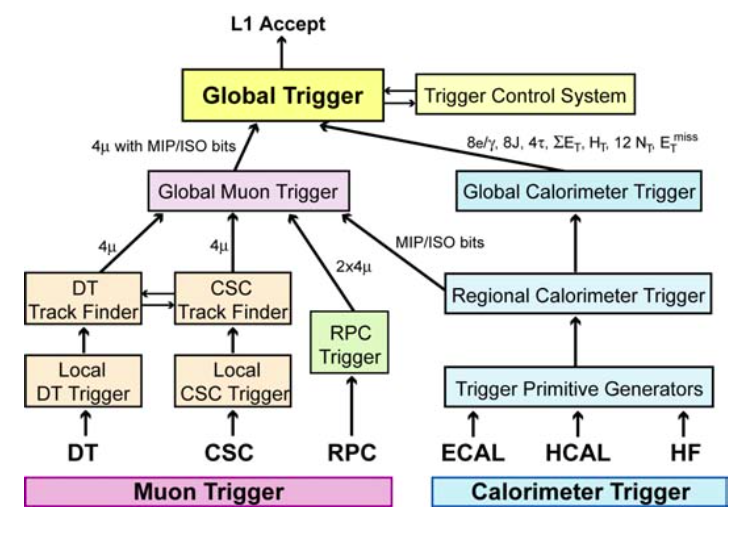
\includegraphics[width=0.65\textwidth]{../figs/l1_organi.png}
    \caption{Organizational chart of the various components of any L1-accept. The two systems (calorimetry and muons) work in parallel 
until they are combined at a regional/global level into the global trigger decision~\cite{cmsdetector}.}
    \label{fig:l1}
\end{figure}
The calorimeter part of the trigger has inputs from the ECAL, HCAL, and the HF, constructing first so-called Trigger Primitives from coarsely organized trigger `towers'. These are
then fed into a regional trigger, where energy sums and crude identifications of physical objects are performed. This information is then given to the global trigger, which constructs
relevant variables such as the total energy deposited, the number of jets, etc.
In parallel, the muon system tries to identify tracks of muons and calculate their \pt by taking information from all three sub-systems and combining it into the Global
Muon trigger. This output is then combined with the calorimeter trigger into a final trigger decision, the aforementioned L1-accept.


The input rate to the L1 is the bunch crossing frequency of the LHC and the maximum processing time of the L1 logic is \SI{3.2}{\micro\second}. The output rate, 
i.e. the rate of L1-accepts, is limited to \SI{100}{\kilo\hertz}. At this rate, the
L1-accept is passed to all the subdetectors, triggering full readout of the event information stored in buffers. This set of complete data is then passed on to the HLT.

\subsubsection*{The HLT}
At the L1 output rate, the full information from the detector is sent from the experimental cavern at P5 to a computer farm situated above ground for further processing.
This computer farm is made of a large number of commercial CPUs (in total about \num{13000}) cores, running reconstruction software which is implemented into the whole 
CMS reconstruction software, package 
described below in section~\ref{sub:cms_reco}, albeit with different sets of parameters optimized for speed~\cite{hltcms, hltcms2}. The HLT starts with L1 information on the candidates for
physical objects, and improves the reconstruction. The organization is done in so-called HLT paths, which are essentially requirements on physical objects being present in
a collision. An example which will be used later on in the analysis part of this thesis is \texttt{HLT\_Mu17\_Mu8\_v1}, which requires the presence of one muon with \pt
greater than 17 \gev and another muon with \pt greater than 8 \gev on HLT level. Other `online' physical objects in the HLT include electrons, jets, missing transverse
energy, and \HT -- the scalar sum of all jet-$p_T$s above a threshold. The reconstruction of objects is divided into modules for any given quantity, followed by a filter on 
the quantity where a cut is applied, in order to save precious computation time of unnecessary quantities. The largest fraction of computation time is taken up by the tracking, and
the total time required for an event depends on the exact event kinematics, up to a limit of \SI{200}{\milli\second}.

The total data reduction factor of the HLT system is roughly \num{10e2}, so the final output rate of events actually fully reconstructed and saved on hard-drives is of the order
of \SI{1}{\kilo\hertz}. About half of this data is reconstructed in the immediate time period after the collision, whereas the other half of the data is first stored and 
reconstructed only later, when computing resources for reconstruction are freed. This process is called data-parking and was implemented for the first time in 2012.

To facilitate analysis of the data when it is fully reconstructed after passing the HLT, different HLT paths are organized in various so-called primary datasets (PDs), which group similar
events into one collection. Examples for primary datasets are DoubleMu, DoubleElectron, and MuEG.

\subsection{Reconstruction and data formats}
\label{sub:cms_reco}
Upon passing the HLT at P5, collision data are sent to the CERN Tier-0 computing center located at the CERN main site in Meyrin for full reconstruction at a rate of roughly \SI{1}{\kilo\hertz}. 
The basic quantity of data in the CMS reconstruction framework -- CMSSW -- is called the `Event', referring to one triggered readout of the full detector. For data analysis it is necessary
to obtain a data format in which physical objects can be identified, this is called the \textit{Event Data Model}, EDM. CMSSW reconstructs different detector related quantities
such as calorimeter energy deposits, tracks from the pixel and strip tracker and muons from the muon chambers, with the best available precision and places those objects into the EDM. 

Tracks are reconstructed using an iterative tracking algorithm where in a first iteration tight criteria for track-seeding are used in order to minimize reconstruction of
fake tracks. In subsequent iterations the set of previously found tracks are used as input, loosening the track fitting requirements to regain tracking efficiency. Five iterations
are done, leading to efficiencies of about 99.5\% for muons, and well above 90\% for charged hadrons within the tracker volume. Tracks with as little as three hits in the ~10 layer
tracker can be reconstructed, with a minimal transverse momentum of about 150 \mev, while the fake rate is kept to below one percent~\cite{pfcms}.

Calorimeter clusters are reconstructed by searching for calorimeter cells with an energy deposit above a certain seed-threshold. These are then combined with adjacent cells
beyond a threshold equivalent to about twice the electronic noise (80-300 \mev in the ECAL and 800 \mev in the HCAL).

Subsequently, these detector-based objects are combined through an algorithm called `Particle Flow' (PF) to identify candidates for physical objects.

\subsubsection*{Particle flow}
The particle flow algorithm~\cite{cmspf} aims at reconstructing an integral picture of every triggered bunch crossing by combining information from all subdetectors to identify
PF candidates. These are photons, electrons, muons, neutral hadrons, and charged hadrons. 

First, tracks are combined with the information from the muon chambers 
to search for `global muons' which have both a track, and are reconstructed in the muon system. If a match is found, this PF muon is put into the appropriate collection in the EDM
and the track is removed from the collection of tracks. The second step involves the matching of tracks and energy clusters in the ECAL, producing a candidate electron. These are then
refit with a Gaussian Sum Filter (GSF) in order to account for bremsstrahlung on the electrons trajectory and the tracks are removed from the track collection. Remaining tracks are
then matched to HCAL deposits to construct a collection of charged hadrons. Any energy deposit that does not have an associated track, is then interpreted as a photon or a neutral
hadron, depending on the energy fractions in the ECAL and HCAL. 

The PF candidates obtained by this algorithm are then taken as the input to the clustering algorithm of hadronic jets. This jet clustering algorithm most widely used in CMS
is the so-called anti-$k_T$ clustering algorithm~\cite{antikt}, developed in 2008. This algorithm is both collinear, and infrared safe\footnote{Collinear safety signifies invariance
of a jet's properties upon division of a constituent's energy into two collinear particles. Infrared safety refers to invariance of the jet upon addition of very soft, i.e. low-energetic,
particles} and the distance parameters of the clustering algorithm are

\begin{align}
    d_{ij} & = \text{min}\left( k_{T,i}^{-2}, k_{T,j}^{-2} \right) \frac{ (\Delta R)^2_{ij}}{R^2}, \\
    d_{iB} & = k_{T,i}^{-2},
    d_{jB} & = k_{T,j}^{-2}.
\end{align}
In this equation, $R$ defines the radial size of a jet, $\Delta R$ is the spacial distance between two candidate particles $i$ and $j$, while $k_{T,i}$ and $k_{T,j}$ are the transverse
momenta of particles $i$ and $j$. If the minimum distance is either $d_{iB}$ or $d_{jB}$, the particle is called a jet and is removed from the collection. Whereas if the minimum distance
is $d_{ij}$, the two particles $i$ and $j$ are merged into a new particle. Because of the inverse exponent in the minimum of the two transverse momenta squared, this means that the 
anti-$k_T$ algorithm clusters soft particles around the hard particles before clustering of soft particles among each other takes place. This leads to perfectly circular jets (as long as
they do not overlap), facilitating corrections to be made due to pileup and other effects.

It is worthwhile to note here, that the PF algorithm in combination with the jet clustering produces overlaps between physical objects. As an example, a muon can enter both the muon
collection and can be reconstructed as a jet. It is therefore important to employ some cross-cleaning of objects in any analysis.

\subsubsection*{Data formats}
Centrally reconstructed events are saved in various data formats all based on EDM, but with differing detail of content. The basic format is RAW, which stored the raw detector information. 
Output from the full reconstruction at the Tier-0 is saved in the RECO data format. This format allows for much flexibility, albeit at very large event sizes, rendering it impractical 
for daily use. The most used format for processing in data analyses is called AOD, Analysis Object Data. This is a simple subset of the RECO data format, containing all relevant information 
for data analysis. The event size of one RECO event is about 1.2 MB, while AOD events are of the order of 300 kB, depending on the kinematics of the event.

Each event is saved at least twice, one copy usually lying at the CERN Tier-0 computing center, and another copy distributed in the LHC Computing Grid (LCG), a worldwide network of computer 
centers for data analysis and storage. Analysis of the data is done with user-written programs running on AOD events. Since primary datasets are of significant size containing oftentimes
many million events at once, these programs are sent by the user via the LCG to a computing center which hosts the dataset of interest, rather than the dataset being copied to the user. The final
data formats used in small-scale analysis are ROOT based files~\cite{root}. ROOT is a data analysis framework conceived especially for data analysis at CERN. It features many convenient 
data formats, such as TTrees\footnote{See \texttt{http://root.cern.ch/root/html/TTree.html} for more details.}, and provides capabilities of producing plots, histograms, perform fits and many 
more functionalities.


\subsection{Simulation and Monte-Carlo}
\label{sub:cms_mc}

